\documentclass[11pt,a4paper]{article}
\usepackage[T1]{fontenc}
\usepackage[utf8]{inputenc}
\usepackage{lmodern}
\usepackage[margin=25mm,headheight=15pt]{geometry}
\usepackage{amsmath,amssymb,amsthm,mathtools,mathrsfs}
\usepackage{microtype,booktabs,longtable,tabularx,array}
\usepackage{xcolor,fancyhdr,enumitem}
\usepackage{tikz}
\usetikzlibrary{arrows.meta,positioning,calc}
\usepackage[unicode,colorlinks=true]{hyperref}
\usepackage{bookmark}
\definecolor{Ink}{HTML}{20354B}
\definecolor{Accent}{HTML}{24656D}
\definecolor{Pale}{HTML}{EDF4F5}
\hypersetup{linkcolor=Ink,citecolor=Accent,urlcolor=Accent,
 pdftitle={From Surcomplex Hahn Fields to Berkovich Geometry},
 pdfauthor={Research exposition prepared for Vladimir Reshetnikov},
 pdfsubject={Rank-one convergence, Tate algebras, analytic annuli, and entire functions}}
\pagestyle{fancy}\fancyhf{}
\fancyhead[L]{\small From surcomplex Hahn fields to Berkovich geometry}
\fancyhead[R]{\small\thepage}
\renewcommand{\headrulewidth}{0.3pt}
\setlength{\parskip}{0.25em}
\setlength{\emergencystretch}{3em}
\setlist{nosep,leftmargin=1.7em}
\allowdisplaybreaks[2]
\numberwithin{equation}{section}
\newtheorem{theorem}{Theorem}[section]
\newtheorem{proposition}[theorem]{Proposition}
\newtheorem{lemma}[theorem]{Lemma}
\newtheorem{corollary}[theorem]{Corollary}
\theoremstyle{definition}
\newtheorem{definition}[theorem]{Definition}
\newtheorem{example}[theorem]{Example}
\theoremstyle{remark}
\newtheorem{remark}[theorem]{Remark}
\newcommand{\No}{\mathbf{No}}
\newcommand{\SC}{\mathbf{SC}}
\newcommand{\C}{\mathbb C}
\newcommand{\R}{\mathbb R}
\newcommand{\Q}{\mathbb Q}
\newcommand{\N}{\mathbb N}
\newcommand{\Z}{\mathbb Z}
\newcommand{\K}{K}
\newcommand{\OO}{\mathcal O}
\newcommand{\mm}{\mathfrak m}
\newcommand{\TT}{\mathcal T}
\newcommand{\PP}{\mathcal P}
\newcommand{\Ag}{\mathcal A}
\newcommand{\FF}{\mathcal F}
\newcommand{\EE}{\mathcal E}
\newcommand{\abs}[1]{\lvert#1\rvert}
\newcommand{\norm}[1]{\lVert#1\rVert}
\newcommand{\vabs}[1]{\lvert#1\rvert_v}
\newcommand{\Gauss}[2]{\lVert#1\rVert_{#2}}
\newcommand{\supp}{\operatorname{supp}}
\newcommand{\red}{\operatorname{red}}
\newcommand{\Res}{\operatorname{Res}}
\newcommand{\dR}{\mathrm{dR}}
\newcommand{\Sp}{\mathcal M}
\newcommand{\id}{\mathrm{id}}
\newcommand{\an}{\mathrm{an}}
\newcommand{\dd}{\,\mathrm d}
\newcommand{\repocommit}{e260237db9b71da8b74a0c13c8e6355119091100}
\newcommand{\repobase}{https://github.com/VladimirReshetnikov/Surreal/blob/e260237db9b71da8b74a0c13c8e6355119091100/}
\newcolumntype{L}{>{\raggedright\arraybackslash}X}
\newcolumntype{P}[1]{>{\raggedright\arraybackslash}p{#1}}

\begin{document}
\hypersetup{pageanchor=false}
\begin{titlepage}
\vspace*{10mm}
{\color{Accent}\large\scshape A continuation of the Surreal repository\par}
\vspace{13mm}
{\color{Ink}\Huge\bfseries From Surcomplex\par Hahn Fields to\par Berkovich Geometry\par}
\vspace{7mm}
{\LARGE Rank-one convergence, Tate algebras,\par analytic annuli, and an entire-function case study\par}
\vspace{10mm}
{\large Research exposition prepared for Vladimir Reshetnikov\par}
{\large September 21, 2026\par}
\vspace{11mm}
\begin{abstract}
The repository develops several support-controlled analytic categories over
surreal and surcomplex numbers, and briefly compares them with Berkovich
geometry. This article fills a different, more concrete gap: it constructs a
rank-one Banach-analytic theory inside the surcomplex field and proves exactly
how it relates to the repository's Hahn-coefficient rings.

Working primarily in $K=\C((t^{\R}))\subset\No[i]$, we distinguish intrinsic
valuation convergence from strong Hahn summability and the full surreal fine
topology. We prove strict comparisons of the function rings, construct one-variable
Weierstrass preparation by a contraction argument, and derive analytic root
counts and a valuation Rouch\'e theorem. We then build the relevant Berkovich
points, explain disks, branches and annulus skeletons, and calculate analytic
de Rham cohomology and residues without pretending that an ultrametric annulus
has an ordinary circular contour.

The case study $F(Z)=\sum_{n\ge0}t^{n^2}Z^n$ has exactly one simple zero of
valuation $-(2m-1)$ for every $m\ge1$, all its zeros are real and negative,
and their first corrections and a convergent canonical product are explicit.
This example also locates the precise boundary between fixed-workspace
entireness and an assertion on the whole proper class $\No[i]$.
\end{abstract}
\vfill
\noindent\colorbox{Pale}{\parbox{\dimexpr\textwidth-2\fboxsep\relax}{\small
\textbf{Status and scope.} A theorem-driven exposition and comparison, not a
claim of first occurrence or the solution of a named open problem. Deep imported
results are identified; the central comparison and computational examples are
proved here. The general arguments are not formally verified. The accompanying
program checks 542 finite exact identities and coefficient assertions.
}}
\end{titlepage}
\hypersetup{pageanchor=true}
\pagenumbering{roman}
\setcounter{tocdepth}{2}
{\small\tableofcontents}
\clearpage
\pagenumbering{arabic}

\section{The documentation gap and the mathematical contract}
\label{sec:gap}

\subsection{What the repository already contains}
The original audit behind this article used the repository snapshot
\begin{center}\small\texttt{\repocommit}\end{center}
from the default branch, inspected on September 21, 2026. It was a targeted
review of the catalogue, the relevant report READMEs, and the introductory and
comparison material in the analytic reports, not a line-by-line certification
of every manuscript or a lexical search asserted to be exhaustive.

The distinction matters because this is not an empty subject in the repository.
The \emph{analysis} report develops infinitesimal and Hahn-coherent function
theory. The \emph{analytic-geometry} report distinguishes ordinary convergent
germs, common-domain coefficient families, and formal coefficients. The
\emph{polynomial-algebra} report gives extensive finite-degree valuation
geometry. Finally, \emph{contours-and-stokes} explicitly compares its integration
categories with Berkovich and tropical approaches
\cite{RepoMap,RepoAnalysis,RepoGeometry,RepoPolynomial,RepoContours}.

At that snapshot the identified gap was \emph{an undeveloped bridge}, rather
than the absence of the word ``Berkovich''. The inspected reports did not
provide a sustained construction of a
rank-one Tate algebra, identify its exact position among their coefficient rings,
and then work through the associated Berkovich disks, analytic annuli and a
nonpolynomial entire function in that category. Those are the tasks undertaken
here. The existing discussions of the intrinsic topology of a Hahn workspace
already avoid identifying it with the topology induced from all of $\No[i]$;
we amplify that correct distinction rather than attribute an error to them.

\begin{center}\small
\begin{tabularx}{\textwidth}{@{}P{0.24\textwidth}LL@{}}
\toprule
Existing report & Existing emphasis & Added here\\\midrule
Analysis & Strong summability and coherent ordinary coefficient functions
 & A complete real-valued norm and actual Banach convergence\\[0.5em]
Analytic geometry & Radius-free and common-domain Hahn germ rings
 & An explicit strict comparison with Tate and open-disk algebras\\[0.5em]
Polynomial algebra & Finite-degree Newton profiles and valuation balls
 & Preparation, root counts and slopes for convergent infinite series\\[0.5em]
Contours and Stokes & Coefficientwise, deformed and algebraic contour pairings;
 category comparisons
 & Berkovich disk points, annulus skeletons and analytic Laurent primitives\\[0.5em]
Foundations & Fixed-workspace versus proper-class scope; a quadratic-exponent
 entire example
 & The complete zero spectrum and product expansion of that example\\
\bottomrule
\end{tabularx}
\end{center}

\subsection{Three questions that must be answered separately}
For a displayed infinite expression, the following are different questions.
Does it define a Hahn sum? Do its partial sums converge in the intrinsic
valuation topology of a specified field? Do they converge when every surreal
scale is allowed as a test of smallness? A positive answer to the first or the
second does not give a positive answer to the third.

Likewise a function ring, a topology on its points, and an integration theory are
separate choices. Our primary objects are Banach algebras over a fixed complete
rank-one valued field. Their spectra are set-sized spaces of seminorms. The
associated differential is differentiation in a coordinate $Z$, fixing the
coefficient field. None of these conventions selects a derivation of the surreal
numbers themselves or defines a contour integral on arbitrary fine-topological
surcomplex paths.

\subsection{Established inputs and the level of proof}
We use the standard Hahn-field construction and the algebraic closedness theorem
for divisible value group and algebraically closed residue field; Poonen's
Corollary 4 supplies a precise reference \cite{Poonen}. The general point
classification and the annulus deformation retraction in Berkovich geometry
are imported from the standard theory \cite{Temkin,PT}. In contrast, the
support and convergence comparisons, the one-variable preparation argument,
root-count formulas, residue computations, and the entire-function case study
are given with proofs in this article.

These are adaptations and deductions in an established subject, not a priority
claim based on replacing ``non-Archimedean'' by ``surcomplex''. In particular,
the worked series is already used in the repository's foundations discussion,
and is a rescaling of the classical partial theta series \cite{RepoFoundations,Sokal}.
What is supplied here is a unified valuation-analytic treatment with its
hypotheses exposed and its finite calculations reproducible.

\section{A complete rank-one field inside the surcomplex numbers}
\label{sec:field}

\subsection{Normal forms and the two meanings of size}
For a set-sized ordered additive subgroup $\Gamma\subset\No$, write
\[
 K_\Gamma=\C((t^\Gamma)),\qquad t^\gamma:=\omega^{-\gamma}.
\]
The last expression is Conway's monomial map. It is not an instruction to use
Gonshor exponentiation with a general surreal exponent. An element is a formal
sum
\begin{equation}\label{eq:hahn}
 a=\sum_{\gamma\in S}c_\gamma t^\gamma,
 \qquad c_\gamma\in\C^*,\quad S\subset\Gamma\text{ well ordered}.
\end{equation}
The zero element has empty support. All supports and all function algebras used
below are sets. Hahn addition and multiplication identify this field with a
subfield of $\No[i]$, with conjugation on the coefficients
\cite{RepoAnalysis,Poonen}.

From now on the main field is
\begin{equation}\label{eq:mainfield}
 K=\C((t^\R)),\qquad
 v(a)=\min\supp(a),\qquad
 \vabs{a}=e^{-v(a)}\quad(a\ne0).
\end{equation}
We put $v(0)=+\infty$ and $\vabs0=0$. Then
\[
 \vabs{ab}=\vabs a\vabs b,
 \qquad \vabs{a+b}\le\max\{\vabs a,\vabs b\}.
\]
The real exponential in \eqref{eq:mainfield} merely turns a real-valued
valuation into a positive real-valued norm. It is \emph{not} a specialization
of the surreal number $t$ to the real number $e^{-1}$.

In particular,
\begin{equation}\label{eq:trivialconstants}
 \vabs c=1\quad(c\in\C^*),\qquad
 \vabs n=\vabs{n!}=1\quad(n\in\N_{>0}).
\end{equation}
The ordinary complex absolute value of a coefficient is irrelevant to this
norm. We reserve $\vabs{\cdot}$ for the valuation norm throughout. The
surreal-valued modulus $\sqrt{x^2+y^2}$ is a different object. Its unit disk,
for example, is not the valuation unit disk: every nonzero ordinary complex
number has valuation norm one.

The valuation ring, maximal ideal and residue field are
\[
 \OO_K=\{a:v(a)\ge0\},\quad
 \mm_K=\{a:v(a)>0\},\quad
 \OO_K/\mm_K\simeq\C.
\]
Reduction $\red$ extracts the coefficient of $t^0$ on $\OO_K$.
Every positive real radius occurs: if $R=e^{-\beta}$, then
$\vabs{t^\beta}=R$. The algebraic closedness of $K$ follows from the cited
Hahn-field theorem because $\R$ is divisible and $\C$ is algebraically closed.
Its real-coefficient subfield $\R((t^\R))$ is consequently real closed.

\subsection{Why this Hahn field is spherically complete}
\begin{definition}
A valued field is \emph{spherically complete} if every nonempty nested family
of nonempty closed valuation balls has nonempty intersection.
\end{definition}

\begin{proposition}\label{prop:spherical}
The field $K=\C((t^\R))$ is spherically complete, and in particular complete
for the metric $d(a,b)=\vabs{a-b}$.
\end{proposition}
\begin{proof}
A ball of positive radius has the form
\[
 B_i=\{x:v(x-a_i)\ge\gamma_i\}.
\]
It prescribes exactly the coefficients of $x$ at exponents strictly below
$\gamma_i$. In a nested family these prescriptions agree wherever both apply:
if one ball is contained in another, its center belongs to the larger ball.
Glue all prescribed coefficients, and set every coefficient not prescribed to
zero.

The support of the glued expression is well ordered. Indeed, let $T$ be a
nonempty subset of that support and choose $s\in T$. Some prescription contains
the coefficient at $s$, so $s<\gamma_i$ for one $i$. All the prescribed
coefficients at exponents at most $s$ agree with $a_i$: a smaller ball agrees
below $\gamma_i$, and a larger ball's prescription agrees with that of $a_i$
where it is defined. Therefore
$T\cap(-\infty,s]$ is a nonempty subset of the well-ordered support of $a_i$.
Its least element is also the least element of $T$.

The glued expression is a Hahn series and satisfies every prescription, hence
belongs to every ball. A ball of radius zero is a singleton and causes no
problem. Finally a Cauchy sequence has a subsequence contained successively in
nested balls with radii tending to zero; an intersection point is its limit and
then the limit of the original sequence.
\end{proof}

This proof uses the full Hahn field, not the completion of finite monomial
expressions. Those need not coincide. For example,
\[
 h=\sum_{n\ge0}t^{1-1/(n+1)}
\]
is a Hahn series, but no finite-support series approximates it with error
valuation greater than one. The infinitely many nonzero coefficients below one
would all have to be matched. In $\C((t^\Q))$, the metric closure of the
finite-support series consists precisely of the series whose support has finite
intersection with $(-\infty,B]$ for every real $B$: necessity follows from
approximation to each cutoff, and sufficiency from finite truncation. The full
Hahn field is larger. Spherical completeness should never be inferred merely
from the word ``completion''.

\subsection{Intrinsic topology versus full surreal topology}
\begin{proposition}\label{prop:topologies}
In the intrinsic valuation topology of $K$, $t^n\to0$. The subspace topology
that $K$ inherits from the full fine topology of $\No[i]$ is discrete, and in
that topology $t^n$ does not converge to zero.
\end{proposition}
\begin{proof}
Intrinsically $\vabs{t^n}=e^{-n}\to0$. In the full surreal field, however,
the positive radius $t^\omega$ is smaller than the surreal modulus of every
nonzero element of $K$: the latter has a real leading exponent, whereas
$\omega$ exceeds every real exponent. Thus the fine ball of radius $t^\omega$
around an element of $K$ meets $K$ only at that element. In particular none of
the $t^n$ belongs to the fine ball of that radius about zero.
\end{proof}

The distinction is a change in topology, not a conflict about the field
operations. The detailed contour report already states the corresponding
workspace qualification \cite{RepoContours}. A theorem about fine convergence
on the full proper class is not a theorem about this intrinsic metric.

\section{Convergence, summability, and the rank-one boundary}
\label{sec:convergence}

\subsection{When an infinite sum really is a limit}
A family of Hahn series is \emph{strongly summable} if the union of its supports
is well ordered and only finitely many members contribute to any specified
exponent. Its sum is then defined coefficientwise. This definition has no
reference to a norm limit.

\begin{theorem}\label{thm:series}
For a sequence $(a_n)$ in $K$, the following are equivalent:
\[
 \sum_{n\ge0}a_n\text{ converges in the intrinsic norm},
 \qquad \vabs{a_n}\longrightarrow0,
 \qquad v(a_n)\longrightarrow+\infty.
\]
When they hold, the family $(a_n)$ is strongly summable and its Hahn sum is the
norm limit. Strong summability alone does not imply any of these conditions.
\end{theorem}
\begin{proof}
Convergence forces the differences of consecutive partial sums to tend to zero.
Conversely, the ultrametric inequality bounds every finite tail by the largest
norm of a term in that tail. Terms tending to zero therefore make the partial
sums Cauchy; Proposition~\ref{prop:spherical} supplies their limit.

Fix an exponent cutoff $B$. Only finitely many $a_n$ have valuation at most
$B$, so the part of the support union at or below $B$ is contained in a finite
union of well-ordered sets. To find the least element of an arbitrary nonempty
subset of the union, choose any one of its elements and use it as this cutoff.
This proves well ordering. A fixed exponent occurs in only finitely many
members for the same reason. Each coefficient stabilizes in the partial sums,
and the stabilized coefficients give the norm limit.

For the failure of the converse take $a_n=t^{1-1/(n+1)}$. Its supports form a
well-ordered increasing sequence, with no repeated exponent, but
$\vabs{a_n}\to e^{-1}$ rather than zero.
\end{proof}

There is a second useful warning in this example: a single Hahn coefficient may
have infinitely many terms below a finite cutoff. Banach convergence of a
sequence of such coefficients does not turn every coefficient into a finite
object or provide an algorithm for accessing its support.

\subsection{Why higher rank cannot be silently scalarized}
\begin{proposition}\label{prop:rankobstruction}
The ordered group $\Q+\Q\omega\subset\No$ has no order-preserving injective
additive map to $\R$. In particular, its natural valuation cannot be converted
faithfully to a real-valued absolute value by an order embedding.
\end{proposition}
\begin{proof}
If $\phi$ were such an embedding, $\phi(1)>0$. But $n<\omega$ for every
positive integer $n$, so $n\phi(1)<\phi(\omega)$ for every $n$, contrary to the
Archimedean property of $\R$.
\end{proof}

A noninjective order-preserving homomorphism can discard an entire layer of
scale; in this example it must kill $1$. Such a coarsening can be useful, but
is not a faithful replacement of the original valuation. The sequence $t^n$
again diagnoses the issue: its valuations are unbounded in $\R$, but are all
below $\omega$ in $\Q+\Q\omega$.

The repository's localization principle puts any given \emph{set} of
surcomplex numbers in some set-sized divisible Hahn workspace
\cite{RepoFoundations}. It does not put every such set in a workspace whose
natural value group has rank one. Already the pair $t,t^\omega$ prevents
that conclusion. Our results therefore concern a substantial subfield, not an
analytic structure transported without loss to every surcomplex scale.

\subsection{Legitimate changes of workspace}
The inclusions
\[
 \C((t^\Q))\ \subset\ \C((t^\R))\ \subset\ \No[i]
\]
have different analytic meanings. The first is isometric for the displayed
real-valued norms. A norm-convergent sequence over the smaller field retains
its limit in the larger rank-one field. The second has no such implication
when the topology on the target is the full fine topology. Conversely, enlarging
$\Q$ to $\R$ fills out the set of available valuation radii; it changes the
types of nonclassical disk points discussed in Section~\ref{sec:berkovich}.

\section{Tate algebras and closed valuation disks}
\label{sec:tate}

\subsection{The coefficient condition is the analytic definition}
Fix $R>0$ and write $R=e^{-\beta}$, $\beta\in\R$. The closed valuation disk
and its Tate algebra are
\begin{align}
 D_R(K)&=\{z\in K:\vabs z\le R\},\label{eq:disk}\\
 A_R=K\langle R^{-1}Z\rangle
 &=\left\{\sum_{n\ge0}a_nZ^n:\vabs{a_n}R^n\longrightarrow0\right\}.
 \label{eq:tate}
\end{align}
The notation $R^{-1}Z$ records the norm assigned to the coordinate; it does not
regard $R$ as a coefficient with that valuation norm. Substitution $Z=t^\beta U$
identifies $A_R$ isometrically with the unit-radius algebra
$\TT=K\langle U\rangle$. Equivalently, the condition in \eqref{eq:tate} is
\begin{equation}\label{eq:tatevaluation}
 v(a_n)+n\beta\longrightarrow+\infty.
\end{equation}

The Gauss norm is
\[
 \Gauss fR=\max_{n\ge0}\vabs{a_n}R^n.
\]
The maximum exists for $f\ne0$ because the terms tend to zero. An infinite
formal expression without the tail condition is not a member of $A_R$ merely
because each of its coefficients lies in $K$.

\begin{proposition}\label{prop:banach}
The algebra $A_R$ is a complete normed $K$-algebra; polynomials are dense;
evaluation at $z\in D_R(K)$ is defined by a norm-convergent series and satisfies
$\vabs{f(z)}\le\Gauss fR$. The Gauss norm is multiplicative.
\end{proposition}
\begin{proof}
The weighted coefficients of a Cauchy sequence converge coordinatewise in $K$.
To check the vanishing-tail condition for its limit, approximate the sequence
uniformly by one member and then discard that member's sufficiently far tail.
This also proves convergence in Gauss norm. Polynomial truncation proves
density. Evaluation and its bound follow from Theorem~\ref{thm:series} and the
ultrametric inequality. Multiplication is the usual Cauchy product, justified
either by the same estimates or by continuous extension from polynomials.

For multiplicativity reduce to $R=1$. Divide each nonzero factor by one of its
coefficients of maximal norm. The normalized series have all coefficients in
$\OO_K$, and their reductions are nonzero polynomials in $\C[U]$: only finitely
many coefficients have norm one. Reduction of the product is the product of
these two polynomials, which is nonzero. The product consequently has norm one,
as claimed after reversing the normalizations.
\end{proof}

\begin{proposition}\label{prop:supnorm}
For every $f\in A_R$,
\[
 \Gauss fR=\max_{z\in D_R(K)}\vabs{f(z)}.
\]
\end{proposition}
\begin{proof}
For $f=0$ the assertion is immediate. Otherwise normalize and scale as in the
preceding proof. Choose $c\in\C$ which is not a
root of the nonzero reduction polynomial. Evaluation at $U=c$ then has norm
one. Such a $c$ exists because $\C$ is infinite. Rescaling proves the result.
\end{proof}

This is a maximum-modulus statement for a valuation norm. It neither selects an
ordinary circular contour nor implies that all functions attain their maxima at
one classical point. A single \emph{nonclassical} point will do that in the
Berkovich spectrum.

\subsection{Two familiar series with different behavior}
The geometric series $\sum_{n\ge0}t^nZ^n$ belongs to $A_1$ and is the inverse
of $1-tZ$ there. Its equality with that inverse is both an algebraic identity and
an intrinsic norm limit. In contrast,
\[
 \sum_{n\ge0}\frac{Z^n}{n!}
\]
does not belong to $A_1$, since every coefficient has norm one. It does belong
to $A_R$ for every $R<1$. Ordinary complex entireness of the coefficient
function $e^Z$ and valuation-analytic entireness in the variable $Z$ are thus
entirely different requirements.

\section{An exact bridge between analytic function rings}
\label{sec:bridge}

\subsection{The rings and the common ambient formal algebra}
Use the same variable $Z$ throughout and put
\begin{align*}
 \TT&=K\langle Z\rangle,&
 \PP&=\C[Z]((t^\R)),\\
 \Ag&=\C\{Z\}((t^\R)),&
 \FF&=\C[[Z]]((t^\R)).
\end{align*}
Here $\C\{Z\}$ is the ordinary complex ring of convergent germs. In $\Ag$
each Hahn coefficient is such a germ, with no common complex radius required.
The symbols $\PP,\Ag,\FF$ demand one well-ordered Hahn support for the whole
family; they are not arbitrary collections of coefficients in $K$.

All four rings map into $K[[Z]]$. To describe the map explicitly write
\[
 H=\sum_{s\in S}h_s(Z)t^s,\qquad
 h_s(Z)=\sum_{n\ge0}c_{s,n}Z^n,
 \qquad b_n=\sum_{s\in S}c_{s,n}t^s.
\]
Then $H$ maps to $\sum b_nZ^n$. Each $b_n$ has support contained in $S$;
coefficient uniqueness makes the map injective. The usual finite decomposition
property for sums of well-ordered supports makes it a ring homomorphism. These
are coefficientwise identities, not a Fubini theorem for arbitrary norm limits.

Finally define the analytic open-unit-disk ring by
\begin{equation}\label{eq:openring}
 \EE^-=
 \left\{\sum_{n\ge0}b_nZ^n\in K[[Z]]:
    v(b_n)+n\varepsilon\to+\infty\text{ for every }\varepsilon>0\right\}.
\end{equation}
It is equivalently the ring of compatible power-series sections on all centered
closed disks of radius less than one. Such disks exhaust the open disk. This
explicit description suffices here; the usual Berkovich analytic interpretation
agrees with it \cite[Section I.4]{PT}.

\subsection{The strict comparison theorem}
\begin{theorem}\label{thm:chain}
Under the preceding coefficient embeddings, the following inclusions of
$K$-algebras inside $K[[Z]]$ are all strict:
\begin{equation}\label{eq:chain}
 K[Z]\ \varsubsetneq\ \TT\ \varsubsetneq\ \PP
 \ \varsubsetneq\ \Ag\ \varsubsetneq\ \FF
 \ \varsubsetneq\ \EE^-.
\end{equation}
Moreover, membership in $\FF$ is equivalent to the union
$\bigcup_n\supp(b_n)$ being well ordered. Within $\FF$, membership in $\PP$
means that every exponent-row $(c_{s,n})_{n\ge0}$ has finite support, and
membership in $\Ag$ means that every such row is an ordinary convergent germ.
\end{theorem}
\begin{proof}
The criterion for $\FF$ follows directly by transposing the coefficient matrix;
its support is exactly the union of the nonzero column supports. The additional
row conditions are precisely the definitions of $\PP$ and $\Ag$.

For $\TT\subset\PP$, use $v(b_n)\to+\infty$. At any fixed exponent only
finitely many columns can contribute, so each row is a polynomial. Below any
fixed exponent cutoff, only finitely many column supports occur. Their union is
well ordered; the least-element argument in Theorem~\ref{thm:series} shows that
the full union is well ordered as well.

For $\FF\subset\EE^-$, a nonzero common support $S$ has a least exponent
$s_0$. Thus $v(b_n)\ge s_0$ for every $n$, and
$v(b_n)+n\varepsilon\ge s_0+n\varepsilon\to+\infty$.
The remaining inclusions are immediate from the coefficient definitions.

The successive strictness witnesses are as follows:
\begin{align*}
 \TT\setminus K[Z]:&\quad \sum_{n\ge0}t^nZ^n,\\
 \PP\setminus\TT:&\quad \sum_{n\ge0}t^{1-1/(n+1)}Z^n,\\
 \Ag\setminus\PP:&\quad \sum_{n\ge0}Z^n/n!,\\
 \FF\setminus\Ag:&\quad \sum_{n\ge0}n!Z^n,\\
 \EE^-\setminus\FF:&\quad \sum_{n\ge0}t^{-\sqrt n}Z^n.
\end{align*}
The second has polynomial exponent-rows but column valuations tending to one,
not to infinity. The third and fourth have the single Hahn exponent zero:
their coefficient functions are respectively a nonpolynomial convergent germ
and a divergent formal series. In the last, $n\varepsilon-\sqrt n\to+\infty$
for every positive $\varepsilon$, but the union of coefficient supports is
unbounded below and hence not well ordered.
\end{proof}

This theorem is the central bridge missing from a mere catalogue of analytic
categories. In particular, $\C[Z]((t^\R))$ is \emph{not} the unit-disk Tate
algebra, even though both may be described informally as series with polynomial
coefficient data. A common Hahn support is a different condition from a
Gauss-norm tail tending to zero.

\subsection{Where the common-domain rings fit}
The two common-domain categories of the repository fit into this comparison as
well. Let $D$ be an ordinary complex open disk centered at zero, and put
\[
 \mathcal H(D)=\OO(D)((t^\R)),\qquad
 \mathcal R_1=\varinjlim_{D\ni0}\mathcal H(D).
\]
The second ring permits one ordinary domain for the entire coefficient family,
followed by shrinking it; it does not permit a different domain for each
coefficient. Taking coefficient Taylor germs gives injections into $\Ag$.
For $\mathcal H(D)$ injectivity uses the ordinary identity theorem on the
connected disk, coefficient by coefficient.

There is the further strict refinement
\begin{equation}\label{eq:domainrefinement}
 \PP\ \varsubsetneq\ \mathcal H(D)\ \varsubsetneq\ \mathcal R_1
 \ \varsubsetneq\ \Ag.
\end{equation}
Every polynomial coefficient is holomorphic on $D$, while the single
coefficient $e^Z$ witnesses the first strictness. For the second, choose
$0\ne b\in D$; the germ of $1/(Z-b)$ is in $\mathcal R_1$ but cannot extend
holomorphically across $b$ on $D$. For the third, use
$\sum_{j\ge1}t^j/(1-jZ)$: its individually convergent coefficient germs have
poles at $1/j$, so no common ordinary neighborhood works. Uniqueness of Hahn
coefficients prevents a different representative from removing these poles.
Thus \eqref{eq:chain} and \eqref{eq:domainrefinement} locate both common-domain
rings without identifying either of them with the Tate algebra.

\subsection{Positive rescaling makes the bridge operational}
\begin{corollary}\label{cor:rescale}
For every $\alpha>0$, substitution $Z=t^\alpha U$ gives an injective
$K$-algebra homomorphism
\[
 \FF\longrightarrow K\langle U\rangle.
\]
Consequently every element of $\Ag$, including a family with no common ordinary
complex radius, becomes a closed-unit-disk Tate function after positive
monomial rescaling.
\end{corollary}
\begin{proof}
With $s_0$ as in the previous proof, the coefficient of $U^n$ has valuation
$v(b_n)+n\alpha\ge s_0+n\alpha\to+\infty$. Formal substitution by a nonzero
scalar is injective and respects products.
\end{proof}

The repository's contour theory uses positive rescaling to obtain
polynomial-coefficient Hahn families \cite{RepoContours}. In rank one the
same lower bound gives the stronger, explicit Banach-tail conclusion above.
For an arbitrary ordered group the step $n\alpha\to+\infty$ need not hold;
Corollary~\ref{cor:rescale} is not being asserted unchanged in higher rank.

For example, the familiar radius-free witness
\[
 H(Z)=\sum_{j\ge1}\frac{t^j}{1-jZ}
\]
has coefficient functions with ordinary poles approaching zero. Nevertheless
$H(t^\alpha U)$ belongs to $K\langle U\rangle$ for every $\alpha>0$.
This does not remove those ordinary complex poles. It changes to an
infinitesimal valuation disk and changes which notion of convergence is being
asked about.

\section{Preparation and zero counting for convergent infinite series}
\label{sec:preparation}

\subsection{Division as a contraction rather than a formal slogan}
The preparation theorem is the point at which an infinite analytic function
acquires finite algebraic control on a fixed closed disk. We give a proof in one
variable, keeping the norm estimates visible. It is the usual non-Archimedean
Weierstrass mechanism in a form suited to the chosen Hahn field, not an appeal
to an unproved preparation theorem for one of the larger rings in
Section~\ref{sec:bridge}.

\begin{lemma}\label{lem:polydivision}
Let $p(U)\in\OO_K[U]$ be monic of degree $d\ge0$. Polynomial division by
$p$ extends to bounded $K$-linear maps
\[
 Q_p:\TT\longrightarrow\TT,\qquad
 R_p:\TT\longrightarrow K[U]_{<d},
\]
with operator norms at most one and
$g=pQ_p(g)+R_p(g)$. Here $K[U]_{<0}=\{0\}$ when $d=0$.
\end{lemma}
\begin{proof}
For a polynomial, ordinary descending-degree division by a monic polynomial
whose other coefficients have norm at most one never increases the largest
coefficient norm. Thus its quotient and remainder are bounded by the norm of
the dividend. Both operators extend continuously from the dense polynomials.
The target of $R_p$ is finite-dimensional and complete; the division identity
passes to the limit. The same continuity argument gives
$Q_p(pq+r)=q$ and $R_p(pq+r)=r$ for $q\in\TT$ and
$r\in K[U]_{<d}$, first on polynomials and then by density.
For $d=0$, $p=1$, the quotient is $g$ and the remainder
zero.
\end{proof}

\begin{theorem}[One-variable Weierstrass division and preparation]
\label{thm:preparation}
Let $0\ne f(U)=\sum a_nU^n\in\TT$, and let
\[
 d=\max\{n:\vabs{a_n}=\Gauss f1\}.
\]
After dividing by $a_d$, suppose $a_d=1$ and $\Gauss f1=1$.
For every $g\in\TT$ there are unique $q\in\TT$ and $r\in K[U]_{<d}$ such
that $g=qf+r$. Moreover
\begin{equation}\label{eq:preparation}
 f=uW,
\end{equation}
where $W\in\OO_K[U]$ is monic of degree $d$ and $u$ is a unit satisfying
$\Gauss{u-1}1<1$. Without the normalization, a nonzero scalar multiplies $u$.
\end{theorem}
\begin{proof}
Write
\[
 p=\sum_{n=0}^d a_nU^n,
 \qquad h=f-p,
 \qquad \theta=\Gauss h1<1.
\]
The strict inequality uses both the choice of the \emph{last} maximal
coefficient and the fact that the tail tends to zero. By
Lemma~\ref{lem:polydivision}, the equation
\begin{equation}\label{eq:divisioncontraction}
 q=Q_p(g-qh)
\end{equation}
is a contraction on the complete normed space $\TT$, with contraction constant
at most $\theta$. Its fixed point exists and is unique. Put $r=R_p(g-qh)$;
then $g=q(p+h)+r=qf+r$.

Conversely any such division must satisfy \eqref{eq:divisioncontraction} upon
applying $Q_p$ to $g-qh=pq+r$. This proves uniqueness. Starting the iteration
at zero also shows $\Gauss q1,\Gauss r1\le\Gauss g1$.

Apply this construction to $g=U^d$. Because $Q_p(U^d)=1$, the fixed point obeys
$\Gauss{q-1}1\le\theta$ and $\Gauss q1=1$. The geometric series shows that
$q$ is a unit with $q^{-1}=1+$ a term of norm less than one. Now
\[
 W=U^d-r=qf
\]
is monic of degree $d$, its coefficients have norm at most one, and
$f=q^{-1}W$ has the asserted form.
\end{proof}

Every invocation of a geometric series or a fixed-point limit in this proof is
in the intrinsic Banach topology. In particular the proof cannot simply be
relabelled as a fine-topological proof over all of $\No[i]$.

\begin{corollary}\label{cor:units}
A series $f\in\TT$ is a unit if and only if
\[
 \vabs{a_0}>\sup_{n\ge1}\vabs{a_n}.
\]
Equivalently $f=a_0(1+h)$ with $\Gauss h1<1$.
\end{corollary}
\begin{proof}
The displayed form is invertible by the convergent geometric series. In the
other direction, normalize $f$ and its inverse and reduce modulo $\mm_K$.
Multiplicativity of the Gauss norm implies that their nonzero reduction
polynomials multiply to a nonzero constant. Both reductions must be constants.
The tail condition then makes the displayed inequality strict.
\end{proof}

\subsection{Finite quotients and one-variable ideal theory}
\begin{corollary}\label{cor:finitequotient}
Every ideal of $\TT=K\langle U\rangle$ is principal. For nonzero $f=uW$ as
in preparation,
\[
 \TT/(f)\simeq K[U]/(W),\qquad
 \dim_K\TT/(f)=\deg W.
\]
Every maximal ideal is $(U-a)$ for a unique $a\in\OO_K$, and its residue
field is $K$.
\end{corollary}
\begin{proof}
In a nonzero ideal choose $f$ with least possible Weierstrass degree. Divide
any other member $g$ by $f$. The remainder is again in the ideal and has
polynomial degree less than that Weierstrass degree. If nonzero, its own
Weierstrass degree is no larger than its polynomial degree, a contradiction.
Thus every remainder is zero and $f$ generates the ideal.

Division by the monic $W$ gives unique polynomial representatives of degree
less than $\deg W$. On polynomials analytic division agrees with ordinary
polynomial division by uniqueness; this proves the asserted quotient
isomorphism. A proper maximal ideal cannot have Weierstrass degree zero.
Since $K$ is algebraically closed, its prepared polynomial factors into linear
terms with roots in $\OO_K$, and maximality forces just one such factor.
Distinct $a$ give distinct evaluation ideals.
\end{proof}

Consequently a finite quotient of the disk algebra is available through
ordinary multiplication matrices, including nonreduced quotients at multiple
zeros. This is a precise one-variable analytic input to the repository's finite
algebra methods. It proves no corresponding ideal theorem for an unnamed
larger function ring merely because its elements also have Hahn coefficients.

There is also a useful warning about the word ``local''. The function on
$\OO_K$ which is zero on $\mm_K$ and one on its complement is locally constant
for the intrinsic ultrametric topology. It is thus locally represented by
constant power series and has derivative zero at every classical point. It is
not a member of $\TT$: any nonzero Tate function has only finitely many zeros
in the closed disk, by preparation and algebraic closedness, whereas this
function has infinitely many zeros and is not identically zero. Arbitrary
pointwise local power-series data in the naive topology are therefore a
larger and less rigid category than functions in a disk Tate algebra.

\subsection{Disk, shell and residue-direction counts}
For $0\ne f(Z)=\sum a_nZ^n\in A_R$ set
\begin{align}
 \lambda_R&=\min_n\bigl(v(a_n)+n\beta\bigr),\notag\\
 m_R&=\min\{n:v(a_n)+n\beta=\lambda_R\},\label{eq:md}\\
 d_R&=\max\{n:v(a_n)+n\beta=\lambda_R\},\notag
\end{align}
where $R=e^{-\beta}$. The normalized initial polynomial is
\begin{equation}\label{eq:initial}
 I_R(U)=\red\left(t^{-\lambda_R}f(t^\beta U)\right)\in\C[U].
\end{equation}
It has degree $d_R$ and order $m_R$ at zero. The normalization is an actual
monomial in $K$, not a norm viewed as a coefficient.

\begin{theorem}\label{thm:rootcounts}
With multiplicities counted, $f$ has exactly $d_R$ zeros in $D_R(K)$, exactly
$m_R$ zeros in $\{\vabs z<R\}$, and exactly $d_R-m_R$ zeros on the shell
$\{\vabs z=R\}$. For each $c\in\C^*$ the number in
\[
 \left\{z\in D_R(K):\red(t^{-\beta}z)=c\right\}
\]
is the multiplicity of $c$ as a root of $I_R$.
\end{theorem}
\begin{proof}
Prepare the scaled series. Its unit factor has no zeros on the closed unit
disk, so all zeros come from a degree-$d_R$ monic polynomial $W$ whose
coefficients have norm at most one. Every root of $W$ has norm at most one:
at a point of norm greater than one its leading monomial strictly dominates all
other terms. Algebraic closedness supplies exactly $d_R$ roots with
multiplicity.

Factor $W=\prod_j(U-u_j)$ in $K[U]$. The $u_j$ lie in $\OO_K$, so
$\red(W)=\prod_j(U-\red(u_j))$. The reduction of the analytic unit is a
nonzero constant, and consequently this polynomial differs from $I_R$ by a
nonzero constant. Roots $u_j$ of norm less than one are exactly those with
reduction zero; roots reducing to a specified nonzero $c$ give the indicated
shell direction. The multiplicities in both descriptions agree.
\end{proof}

The finite-degree initial-polynomial identity in the repository's polynomial
report has thus acquired an analytic justification for infinite series:
Weierstrass preparation makes the extra tail harmless \emph{under an explicit
Gauss convergence condition}. A formal series in $K[[Z]]$ with no such condition
is outside this theorem.

\begin{corollary}[Valuation Rouch\'e theorem]\label{cor:rouche}
If $f,g\in A_R$ and $\Gauss{g-f}R<\Gauss fR$, then $f$ and $g$ have the same
closed-disk, open-disk, shell and residue-direction zero counts at radius $R$.
\end{corollary}
\begin{proof}
The normalized reductions in \eqref{eq:initial} are identical, since the
normalized difference has Gauss norm less than one. Apply
Theorem~\ref{thm:rootcounts}.
\end{proof}

The conclusion protects counts, not labels, equality of roots, or equality of
all the pairwise distances in a cluster. Finer root-matching assertions need
separation hypotheses. Nor does this statement evaluate $f$ and $g$ on an
ordinary complex circle and compare their ordinary complex magnitudes.

\subsection{A simple residual root gives an actual analytic root}
\begin{lemma}[Unit-derivative Hensel lifting]\label{lem:hensel}
Let $f\in\OO_K\langle U\rangle$, $a\in\OO_K$, and suppose
$\vabs{f(a)}<1$ and $\vabs{f'(a)}=1$. There is exactly one root $b$ of $f$ in
$a+\mm_K$. Newton iteration from $a$ converges to $b$; each new residual norm is at most the square of the preceding one.
\end{lemma}
\begin{proof}
Taylor expansion about any point of $\OO_K$ has coefficients in $\OO_K$;
this follows first for polynomials from the integral binomial coefficients,
and then for Tate series by continuity. A displacement $u$ of norm less than
one changes the derivative by a term of norm less than one. The Newton
correction $-f(a)/f'(a)$ therefore has norm less than one, the next derivative
remains a unit, and the Taylor remainder is bounded by the square of the
correction. Iteration gives a Cauchy sequence, hence a root. If $b_1,b_2$ are
in the same residual disk, the divided difference
$(f(b_1)-f(b_2))/(b_1-b_2)$ is a unit when $b_1\ne b_2$; its leading term is
$f'(a)$. It cannot vanish, so two roots there are impossible.
\end{proof}

\section{Berkovich disks: points that are not surcomplex numbers}
\label{sec:berkovich}

\subsection{The spectrum of a Banach algebra}
For $A_R$ define $\Sp(A_R)$ to be the set of maps
$p:A_R\to\R_{\ge0}$ satisfying
\[
 p(0)=0,\quad p(1)=1,\quad p(fg)=p(f)p(g),\quad
 p(f+g)\le\max\{p(f),p(g)\},
\]
which extend $\vabs{\cdot}$ on $K$ and obey $p(f)\le\Gauss fR$.
The topology is the weakest one in which every real-valued map $p\mapsto p(f)$
is continuous. This is the Berkovich closed disk, with the usual bounded
multiplicative-seminorm definition specialized to our algebra
\cite[Definition 2.2.2.1]{Temkin}.
Using the bound with constant one loses no seminorms: if
$p(f)\le C\Gauss fR$ for some fixed $C$, then multiplicativity gives
$p(f)^n=p(f^n)\le C(\Gauss fR)^n$ for every positive integer $n$.
Taking $n$th roots and letting $n\to\infty$ gives $p(f)\le\Gauss fR$.

A classical point $z\in D_R(K)$ gives $p_z(f)=\vabs{f(z)}$. These are not all
points. The Gauss norm itself is a multiplicative seminorm by
Proposition~\ref{prop:banach}, so it defines a point $\zeta_{0,R}$.

\begin{proposition}\label{prop:compact}
The space $\Sp(A_R)$ is nonempty, compact and Hausdorff. Its Gauss point
simultaneously realizes the Gauss norm of every function.
\end{proposition}
\begin{proof}
Embed it in the product
\[
 \prod_{f\in A_R}[0,\Gauss fR].
\]
This is a set-indexed product of compact Hausdorff intervals. The equations and
inequalities defining a seminorm, and the equations on constants, are closed
conditions on its coordinates. Hence $\Sp(A_R)$ is a closed subspace of that
compact Hausdorff product. It is nonempty because it contains evaluation at
zero. At the Gauss point the coordinate $p(f)$ is, by definition, $\Gauss fR$.
\end{proof}

A one-point boundary on which all spectral suprema are attained is thus
available. In the terminology of affinoid algebras, the Gauss point is the
Shilov boundary of the closed disk. No classical point can do this job for every
function. For instance, on the unit disk the Gauss norm of $Z-a$ is one for
every $a\in\OO_K$, while evaluation at $a$ makes it zero. The new point
$\zeta_{0,1}$ is a seminorm, not an exotic surreal number waiting to be named.

\subsection{Disk points and the simplification for the full Hahn field}
For $a\in K$ and $r\ge0$, define a seminorm on $K[Z]$ by
\begin{equation}\label{eq:diskpoint}
 \abs{P}_{a,r}
 =\max_n\vabs{b_n}r^n,
 \qquad P(Z)=\sum_n b_n(Z-a)^n.
\end{equation}
At $r=0$ this is evaluation at $a$. For $r>0$, scale the coordinate by an
 element of norm $r$ and use the reduction proof of multiplicativity. If
$\vabs a\le R$ and $r\le R$, it extends continuously to $A_R$ and defines
$\zeta_{a,r}\in\Sp(A_R)$.

The standard classification over an algebraically closed complete valued field
has four types: classical points; disk points whose positive radius belongs to
the value group; disk points with radius outside it; and points arising from
nested disks with empty intersection. This classification is imported, not
proved merely by drawing a tree
\cite[Lemma I.2.11, Proposition I.2.12 and Remark I.2.13]{PT}.

\begin{corollary}\label{cor:types}
Over $K=\C((t^\R))$ the Berkovich affine line has only types 1 and 2.
Every point is represented by some $\zeta_{a,r}$, with $r\ge0$.
Over $\C((t^\Q))$ types 1, 2 and 3 occur, but type 4 still does not occur.
\end{corollary}
\begin{proof}
For $K$, every positive real radius is in the value group, excluding type 3;
spherical completeness excludes type 4. The coefficient-gluing proof of
Proposition~\ref{prop:spherical} also works over the divisible subgroup $\Q$,
so type 4 is excluded there too. But a radius such as $e^{-\sqrt2}$ is not in
$e^{-\Q}$, and its disk seminorm is of type 3 over that field.
\end{proof}

The distinction between the full Hahn field and its smaller metric subfields
is therefore geometrically visible. An assertion about the types over a
completed Puiseux field must not be copied unchanged to a spherically complete
Hahn field.

\subsection{Where paths come from}
For fixed $a$, the map $r\mapsto\zeta_{a,r}$ is continuous. On polynomials this
follows immediately from \eqref{eq:diskpoint}; on a fixed disk, uniform
polynomial approximation gives the same conclusion for Tate functions.
Moreover,
\begin{equation}\label{eq:equaldisk}
 \zeta_{a,r}=\zeta_{b,r}
 \quad\Longleftrightarrow\quad \vabs{a-b}\le r
 \qquad(r>0).
\end{equation}
One direction follows by recentering and the ultrametric inequality; for the
other evaluate $Z-a$ at the two seminorms.

Two distinct classical points $a,b$ can consequently be joined by increasing
the radius from zero to $d=\vabs{a-b}$ about $a$, then decreasing it from $d$
to zero about $b$. The two radius paths meet at their first common containing
disk. This path uses nonclassical points. It is not a continuous ordinary-real
path taking its values only in the ultrametric field $K$.

More generally for positive-radius disk points $x=\zeta_{a,r}$ and
$y=\zeta_{b,s}$, put
\[
 M=\max\{r,s,\vabs{a-b}\}.
\]
Their common upper disk is $\zeta_{a,M}=\zeta_{b,M}$, and the logarithmic
length of the intervening tree segment is
\begin{equation}\label{eq:treedistance}
 d_{\mathrm{tree}}(x,y)=2\log M-\log r-\log s.
\end{equation}
This is the path-length convention on nonclassical segments, not a claim that
the entire compact weak topology is this metric. Classical endpoints have
infinite logarithmic distance from a fixed positive-radius point even though
the radius-parameterized path reaches them continuously. Unique arcwise
connectedness is a standard theorem of the Berkovich line
\cite[Sections I.6 and I.8]{PT}; the formulas here describe those arcs in the
particular field where every point is a disk point.

\begin{figure}[htbp]
\centering
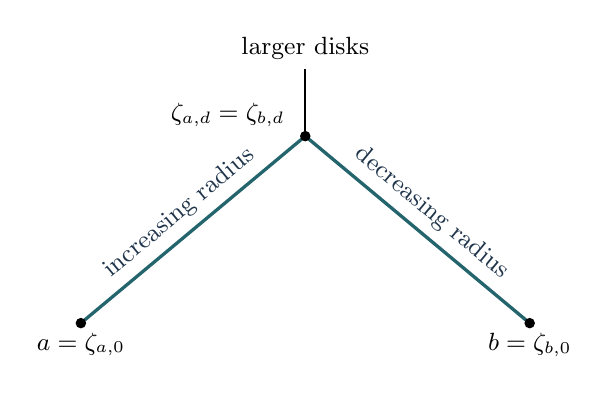
\begin{tikzpicture}[scale=0.95,every node/.style={font=\small}]
\coordinate (a) at (-3,0);\coordinate (b) at (3,0);
\coordinate (m) at (0,2.5);
\draw[very thick,Accent] (a)--node[midway,above,sloped,text=Ink] {increasing radius} (m)
 --node[midway,above,sloped,text=Ink] {decreasing radius} (b);
\draw[thick] (m)--(0,3.4);
\fill (a) circle (2pt) node[below] {$a=\zeta_{a,0}$};
\fill (b) circle (2pt) node[below] {$b=\zeta_{b,0}$};
\fill (m) circle (2pt) node[above left,xshift=-4pt] {$\zeta_{a,d}=\zeta_{b,d}$};
\node[above] at (0,3.4) {larger disks};
\end{tikzpicture}
\caption{A schematic path through the first common disk, with
$d=\vabs{a-b}$. Only the two selected branches and their common upper segment are shown;
this is not an ordinary picture of points in a complex disk.}
\label{fig:tree}
\end{figure}

\subsection{Residue directions replace the circle of boundary points}
The Gauss point of the unit disk has one inward branch for each residue class
$c\in\C$. The corresponding open disk is
\[
 D^-(c,1)=\{x:\abs{Z-c}_x<1\}.
\]
The Berkovich closed unit disk is the disjoint union of its Gauss point and
these open disks. One can see the set decomposition directly in our disk
model: a proper disk of radius less than one has a unique residue center;
a disk of radius one with center in $\OO_K$ is the Gauss point itself.
The standard tree topology makes these precisely the connected branches.
In the projective line there is also the outward direction, giving the
indexing set $\mathbb P^1(\C)$ \cite[Sections I.3 and I.8]{PT}.

This explains the initial polynomial in \eqref{eq:initial}: its roots specify
which residue branches contain zeros and with what multiplicities. The finite
root geometry is no longer an isolated algebraic construction; it is the branch
geometry of an analytic spectrum. Nevertheless its ``boundary'' is not a
circle parametrized by an ordinary angle.

\section{Norm profiles, integer slopes, and a Jensen formula}
\label{sec:slopes}

\subsection{The Newton profile as a function on a radial segment}
Suppose $0\ne f=\sum a_nZ^n$ is analytic on all disks in a nonempty interval of
radii. For $x=\log R$ put
\begin{equation}\label{eq:profile}
 L_f(x)=\log\Gauss f{e^x}
       =\max_{n:a_n\ne0}\{-v(a_n)+nx\}.
\end{equation}
It is also the logarithm of $f$ evaluated at the radial Berkovich point
$\zeta_{0,e^x}$.

\begin{proposition}\label{prop:slopes}
On every compact subinterval of an open interval of analyticity, $L_f$ is the
maximum of finitely many affine functions with nonnegative integer slopes.
It is therefore convex and piecewise affine. At a radius $R=e^x$ where both
one-sided neighborhoods are available,
\[
 L_f'(x-)=m_R,\qquad L_f'(x+)=d_R.
\]
Its slope jump is the number of zeros on the valuation shell of radius $R$,
counted with multiplicity.
\end{proposition}
\begin{proof}
At the largest radius in a compact interval the weighted coefficient norms
tend to zero, and hence the far tail is uniformly small at every smaller
radius in the interval. One fixed nonzero term has a positive minimum norm on
that interval. Eventually every tail term is smaller than that minimum, so it
cannot attain the maximum. Only finitely many affine functions remain.

At an intersection of finitely many active affine functions the left slope of
their maximum is the smallest active slope and the right slope is the largest.
These are exactly the indices in \eqref{eq:md}. The shell count is
Theorem~\ref{thm:rootcounts}.
\end{proof}

At the outer boundary of a domain the algebraic numbers $m_R,d_R$ still make
sense even when a right derivative has no domain. This minor qualification
prevents an implicit analytic continuation assumption.

\subsection{A product formula on a disk}
For a polynomial $P=c\prod_j(Z-\alpha_j)$, multiplicativity gives immediately
\begin{equation}\label{eq:polynorm}
 \Gauss PR=\vabs c\prod_j\max\{R,\vabs{\alpha_j}\}.
\end{equation}
A nonpolynomial Tate function has a similar formula after preparation, its
unit contributing a constant norm on the disk.

\begin{theorem}[Valuation Jensen formula]\label{thm:jensen}
If $f\in A_R$ and $f(0)\ne0$, and $\alpha_1,\ldots,\alpha_d$ are its zeros
in $D_R(K)$ with multiplicity, then
\begin{equation}\label{eq:jensen}
 \log\Gauss fR-\log\vabs{f(0)}
   =\sum_{j=1}^d\log\frac{R}{\vabs{\alpha_j}}.
\end{equation}
A zero on the boundary shell contributes zero to the displayed sum.
\end{theorem}
\begin{proof}
Prepare $f$ after scaling to the unit disk. The unit criterion gives
$\Gauss uR=\vabs{u(0)}$ for its unit factor. Apply
\eqref{eq:polynorm} to the prepared polynomial; all its roots have norm at most
$R$. Divide by the product formula at zero and take real logarithms.
\end{proof}

No angular average occurs in this proof. Formula~\eqref{eq:jensen} is a
statement about the Gauss norm and root radii, and its differentiation along a
radial tree segment gives the integer-slope count. It should not be identified
with the order-modulus Jensen theorem in the repository's polynomial report:
that theorem concerns a different geometry \cite{RepoPolynomial}.

\section{Differentiation, primitives, and a local differential equation}
\label{sec:differential}

\subsection{The coefficient field is held fixed}
The differential in this article is
\[
 \frac{\mathrm d}{\mathrm dZ}\left(\sum a_nZ^n\right)
   =\sum_{n\ge1}n a_nZ^{n-1},\qquad a_n\in K.
\]
Thus $\mathrm dt/\mathrm dZ=0$. It is not a derivation on $\No$ with a chosen
value on $\omega$, and no compatibility with a surreal differential-field
structure is asserted. This is the coordinate differential used for analytic
functions over a fixed ground field.

\begin{proposition}\label{prop:primitive}
For every $R>0$, differentiation is a bounded map $A_R\to A_R$, and
\[
 \Gauss{f'}R\le R^{-1}\Gauss fR.
\]
The zero-constant primitive
\begin{equation}\label{eq:primitive}
 Jf=\sum_{n\ge0}\frac{a_n}{n+1}Z^{n+1}
\end{equation}
belongs to $A_R$, satisfies $(Jf)'=f$, and obeys
$\Gauss{Jf}R=R\Gauss fR$. Consequently the global analytic de Rham complex on
the disk has
\[
 H^0_{\dR}(A_R)=K,\qquad H^1_{\dR}(A_R)=0.
\]
\end{proposition}
\begin{proof}
Every nonzero integer and its inverse have valuation norm one. The displayed
bounds follow term by term from the Gauss norm, and the same estimates preserve
the vanishing tails. The kernel of differentiation consists exactly of the
constants, since the characteristic is zero, and \eqref{eq:primitive} proves
surjectivity. Here $H^1_{\dR}(A_R)$ means the quotient $A_R\dd Z/\mathrm dA_R$
of global analytic forms, which is all that is needed below.
\end{proof}

The norm-one denominator property is essential. In a field with nontrivial
$p$-adic norm on the integers, division by $n+1$ can destroy convergence at the
boundary of a closed disk. Nothing in Proposition~\ref{prop:primitive} is a
blanket assertion for all complete non-Archimedean fields.

\subsection{Why having primitives does not solve every equation globally}
Consider $y'=y$, $y(0)=1$. Coefficient comparison forces the unique formal
solution $y=\sum Z^n/n!$. It is not in $A_1$, although every individual
function of $A_1$ has a primitive in $A_1$. Solving a differential equation is
not the same operation as taking one primitive; infinitely many successive
integrations require their own convergence estimate.

There is a clean local replacement. Give matrices over $A_R$ the maximum-entry
Gauss norm, which is submultiplicative by the ultrametric inequality.

\begin{proposition}\label{prop:ode}
If a matrix $B(Z)$ over $A_R$ satisfies $R\Gauss BR<1$, the initial-value
problem
\[
 Y'=BY,\qquad Y(0)=I
\]
has a unique solution over $A_R$. It satisfies $\Gauss{Y-I}R<1$ and is an
invertible matrix over $A_R$.
\end{proposition}
\begin{proof}
The map $Y\mapsto I+J(BY)$ is a contraction, with constant at most
$R\Gauss BR$. Its fixed point is a solution. Differentiation and evaluation at
zero show that any other solution is the same fixed point. Iterating from $I$
gives $\Gauss YR\le1$ and $\Gauss{Y-I}R\le R\Gauss BR<1$; the matrix
geometric series in $I-Y$ supplies the inverse.
\end{proof}

The condition is sufficient, not necessary. Applied after shrinking a disk on
which $B$ is analytic, it gives a genuinely local existence theorem. It neither
produces a fundamental matrix on every closed disk nor supports a universal
surreal exponential at arbitrary scales.

\section{Analytic annuli, residues, and the failure of a naive comparison}
\label{sec:annuli}

\subsection{Laurent series on a closed annulus}
Fix $0<r<R$. Define
\begin{equation}\label{eq:annulus}
 A[r,R]=\left\{\sum_{n\in\Z}a_nZ^n:
 \begin{array}{ll}
  \vabs{a_n}R^n\to0& (n\to+\infty),\\
  \vabs{a_n}r^n\to0& (n\to-\infty)
 \end{array}\right\}.
\end{equation}
Its norm is
\[
 \Gauss f{[r,R]}=
 \max\left\{\sup_n\vabs{a_n}r^n,\ \sup_n\vabs{a_n}R^n\right\}.
\]
This is a complete submultiplicative norm: the algebra is the completion of
Laurent polynomials for the maximum of their two endpoint Gauss norms. It is
\emph{not generally multiplicative}. Indeed the norms of $Z$ and $Z^{-1}$
are $R$ and $r^{-1}$, while their product is one. Evaluation converges on
$r\le\vabs z\le R$; the two endpoint estimates justify the Cauchy product.

If $a,b\in K^*$ have norms $R,r$, the coordinates $U=Z/a$ and $V=b/Z$
satisfy $UV=b/a$. Thus \eqref{eq:annulus} is the usual annulus affinoid algebra,
also written $K\langle R^{-1}Z,rZ^{-1}\rangle$, with the familiar presentation
$K\langle U,V\rangle/(UV-b/a)$ \cite[Section 3]{Temkin}.

The Laurent coefficients are intrinsic to the analytic function, not just to a
chosen notation. To see injectivity of evaluation, take a nonzero Laurent
series and a radius $\rho\in[r,R]$. After scaling and normalization its
reduction is a nonzero Laurent polynomial. Choose a nonzero complex residue
which is not a root; evaluation at the corresponding point of norm $\rho$
is nonzero. This is the same finite initial-polynomial test used on a disk.

\subsection{The residue is the complete primitive obstruction}
\begin{definition}
For an analytic one-form on the annulus define
\[
 \Res_{[r,R]}\left(\sum_{n\in\Z}a_nZ^n\dd Z\right)=a_{-1}.
\]
The coordinate $Z$ includes an orientation of the annulus: reversing it by
$Z=W^{-1}$ reverses the residue.
\end{definition}

\begin{theorem}\label{thm:annulusderham}
An analytic one-form $f(Z)\dd Z$ on $A[r,R]$ has an analytic primitive on that
same closed annulus if and only if its residue is zero. More precisely,
\begin{equation}\label{eq:exactresidue}
 0\longrightarrow K\longrightarrow A[r,R]
 \xrightarrow{\mathrm d} A[r,R]\dd Z
 \xrightarrow{\Res_{[r,R]}}K\longrightarrow0
\end{equation}
is exact. In particular
$H^1_{\dR}(A[r,R])=K[\mathrm dZ/Z]$.
\end{theorem}
\begin{proof}
A derivative has no $Z^{-1}$ coefficient, so a primitive forces zero residue.
Conversely, when $a_{-1}=0$ set
\[
 P(Z)=\sum_{n\ne-1}\frac{a_n}{n+1}Z^{n+1}.
\]
At each endpoint $\rho=r,R$ the corresponding term norm is
$\rho\vabs{a_n}\rho^n$, since $\vabs{n+1}=1$. Both tails still tend to zero,
so $P$ belongs to the same annulus algebra and $P'=f$.
Its norm is at most $R\Gauss f{[r,R]}$. Constants are the derivative kernel;
the residue is onto because $c\,\mathrm dZ/Z$ has residue $c$.
\end{proof}

The repository already discusses the formal residue quotient
$K((Z))\dd Z/\mathrm dK((Z))$ \cite{RepoContours}. The point here is an analytic
statement with \emph{both} Laurent tails present and convergence preserved on
the very same closed annulus. No shrinking is hidden in the primitive formula.

\begin{proposition}\label{prop:residuepullback}
Under a monomial covering $Z=cW^m$, $c\ne0$, $m\in\N_{>0}$, choose the source
annulus so that $r\le\vabs c\vabs W^m\le R$. Then
\[
 \Res\bigl((cW^m)^*(f(Z)\dd Z)\bigr)=m\Res(f(Z)\dd Z).
\]
Also, if $\Gauss u{[r,R]}<1$, the Banach series
$\log(1+u)=\sum_{k\ge1}(-1)^{k+1}u^k/k$ converges, and
$\Res\bigl(\mathrm d\log(1+u)\bigr)=0$.
\end{proposition}
\begin{proof}
The pullback of a monomial is
$a_n m c^{n+1}W^{m(n+1)-1}\dd W$; exponent $-1$ occurs precisely at $n=-1$.
The annulus endpoint conditions justify passing through the convergent series.
For the logarithm, $\vabs k=1$ and the term norms are bounded by
$\Gauss u{[r,R]}^k\to0$. Differentiation is bounded on the annulus, so it
commutes with the norm limit. Exactness in \eqref{eq:exactresidue} then gives
zero residue.
\end{proof}

\subsection{The Berkovich annulus is contractible, nevertheless}
Let $X[r,R]$ be the Berkovich annulus
\[
 \{x:r\le\abs Z_x\le R\}.
\]
Its skeleton is the interval of disk points
\begin{equation}\label{eq:skeleton}
 \Sigma[r,R]=\{\zeta_{0,\rho}:r\le\rho\le R\}.
\end{equation}
The general deformation-retraction theorem is standard: the open-annulus
construction in \cite[Lemma I.7.9 and Proposition I.7.11]{PT} restricts to
the inverse image of a closed skeleton interval, giving a closed annulus.
For our spherically complete algebraically closed field it has an explicit
proof worth recording.

\begin{proposition}\label{prop:annuluscontract}
The space $X[r,R]$ strongly deformation retracts onto $\Sigma[r,R]$ and is
therefore contractible.
\end{proposition}
\begin{proof}
By Corollary~\ref{cor:types}, each point can be written as $x=\zeta_{a,s}$.
Choose the representation with $s\le\vabs a$; a skeleton point of radius $s$
can be recentered at any $a$ of norm $s$. Then
$\rho=\abs Z_x=\vabs a\in[r,R]$. For $0\le\tau\le1$ define
\[
 H(\tau,x)=\zeta_{a,\max\{s,\tau\rho\}}.
\]
Changing a representing center by distance at most $s$ does not change any of
the enlarged disks, so the map is well defined. It stays in the annulus,
starts at $x$, and ends at
$\zeta_{a,\rho}=\zeta_{0,\rho}$. Skeleton points remain fixed.

For joint continuity it suffices first to test linear polynomials:
\[
 \abs{Z-b}_{H(\tau,x)}
   =\max\{\abs{Z-b}_x,\tau\abs Z_x\}.
\]
This is continuous in $(\tau,x)$. Every polynomial factors into linear terms
because $K$ is algebraically closed, so multiplicativity gives continuity for
all polynomials. Laurent polynomials follow by division by powers of $Z$,
whose norm remains bounded below by $r$. Every annulus function is a uniform
limit of Laurent polynomials, and all these seminorms are bounded by the
annulus norm. Continuity follows for the defining coordinates of the spectrum.
Finally $\rho\mapsto\zeta_{0,\rho}$ identifies the skeleton with $[r,R]$,
with continuous inverse $x\mapsto\abs Z_x$. The interval is contractible.
\end{proof}

Combining this proposition with Theorem~\ref{thm:annulusderham} gives
\begin{equation}\label{eq:comparisonfailure}
 H^1_{\mathrm{sing}}(X[r,R];K)=0,
 \qquad
 H^1_{\dR}(A[r,R])\simeq K.
\end{equation}
There is no contradiction. The analytic differential forms over $K$ used here
are not the real differential forms on the underlying tree-like topological
space. An ordinary complex de Rham comparison cannot be assumed in this new
category. In particular $\mathrm dZ/Z$ has a nonzero analytic residue although
there is no topological loop around a hole in this Berkovich annulus. This is a
concrete reason not to regard the skeleton as an ordinary circular contour.

\subsection{An argument principle with no hidden contour}
Suppose a rational function $f\in K(Z)^*$ has no zero or pole on the closed
annulus. Factoring it gives
\[
 \frac{f'}f=
 \sum_j\frac{m_j}{Z-\alpha_j}
 -\sum_k\frac{n_k}{Z-\beta_k}.
\]
A root or pole has norm either less than $r$ or greater than $R$. If
$\vabs\alpha<r$, then
\[
 (Z-\alpha)^{-1}=\sum_{k\ge0}\alpha^kZ^{-k-1}
\]
converges in the annulus algebra and has residue one. If $\vabs\alpha>R$,
expanding in $Z/\alpha$ gives no negative power and residue zero. Consequently
\begin{equation}\label{eq:argument}
 \Res_{[r,R]}\left(\frac{f'}f\dd Z\right)
 =\#\{\text{zeros in }\vabs z<r\}
  -\#\{\text{poles in }\vabs z<r\},
\end{equation}
with multiplicities. This is an exact Laurent-series argument principle; it
has not been defined as a Riemann integral along a $K$-valued circle.

For a Tate function analytic on a larger disk and nonvanishing on the annulus,
preparation gives the analogous formula. The polynomial factor contributes
its inner zeros; the disk-analytic unit has logarithmic derivative analytic on
the full disk and hence zero annular residue. This version will apply to the
nonpolynomial example in Section~\ref{sec:theta}.

\subsection{Actual, annular, and cluster residues}
Let $\varepsilon\in\mm_K\setminus\{0\}$. The rational form
$\mathrm dZ/(Z-\varepsilon)$ has local residue zero at the actual point $Z=0$
and local residue one at $Z=\varepsilon$. On any annulus with
$\vabs\varepsilon<r<R$ its Laurent residue is one. The Hahn expansion
\[
 \frac1{Z-\varepsilon}
 =\sum_{n\ge0}\varepsilon^nZ^{-n-1}
\]
also has coefficientwise cluster residue one at the ordinary center zero, in
the overlapping rational framework of the repository. These answers agree
where their definitions concern the same cluster, and differ where they concern
different actual points. There is no single symbol ``residue at zero'' that
may safely replace all three constructions.

\section{Entire functions and their canonical products}
\label{sec:entire}

\subsection{Entireness means every real valuation radius}
Define
\begin{equation}\label{eq:entire}
 \EE(K)=\bigcap_{R>0}A_R
 =\left\{\sum_{n\ge0}a_nZ^n:
 v(a_n)+n\beta\to+\infty\text{ for every }\beta\in\R\right\}.
\end{equation}
The intersection is taken inside $K[[Z]]$. Elements are analytic at every
point of this rank-one field. This is not the assertion that the same defining
sum can be evaluated at every point of $\No[i]$.

\begin{theorem}[Growth and zero-free rigidity]\label{thm:liouville}
Let $f\in\EE(K)$.
\begin{enumerate}
\item If $\vabs{f(z)}\le M$ for every $z\in K$ and some real $M$, then $f$ is
constant.
\item More generally, if $\Gauss fR\le C R^d$ for all sufficiently large $R$,
where $d\in\N$, then $f$ is a polynomial of degree at most $d$.
\item If $f$ is zero-free on $K$, then $f$ is a nonzero constant.
\end{enumerate}
\end{theorem}
\begin{proof}
By Proposition~\ref{prop:supnorm}, the first hypothesis bounds every Gauss norm
by $M$. Thus $\vabs{a_n}R^n\le M$ for all $R$, forcing $a_n=0$ for $n>0$.
For the second assertion the same coefficient bound reads
$\vabs{a_n}\le C R^{d-n}$, and letting $R\to\infty$ eliminates $n>d$.

For the third assertion, root counting gives $d_R=0$ at every radius.
In particular $a_0\ne0$ and its term dominates all higher terms at every
radius. A nonzero $a_n$ with $n>0$ would satisfy
$\vabs{a_n}R^n>\vabs{a_0}$ at some sufficiently large radius, a contradiction.
\end{proof}

Zero-free entire rigidity is stronger than bounded-entire rigidity here. It is
not a claim about ordinary complex entire functions: the usual exponential is
excluded from \eqref{eq:entire}. The following product theorem also shows that
a nonpolynomial valuation-entire function must have infinitely many zeros
escaping to infinity in valuation norm.

\subsection{An infinite product without exponential correction factors}
\begin{theorem}\label{thm:canonicalproduct}
Let $0\ne f\in\EE(K)$ have a zero of order $m$ at zero, and let
$(\alpha_j)$ be its nonzero zeros, repeated with their multiplicities.
There are finitely many in each bounded valuation disk, so in the infinite
case they can be enumerated with $\vabs{\alpha_j}\to\infty$. Then
\begin{equation}\label{eq:canonicalproduct}
 f(Z)=cZ^m\prod_j\left(1-\frac Z{\alpha_j}\right),
 \qquad c=[Z^m]f.
\end{equation}
The product converges in $A_R$ for every $R>0$, and its limit is independent
of the escaping enumeration. A nonzero entire function with only finitely
many zeros is a polynomial.
\end{theorem}
\begin{proof}
Theorem~\ref{thm:rootcounts} gives finiteness on each disk. The disks of
radii $e^n$, $n\ge0$, cover $K$, so the zero multiset is countable and can be
enumerated as stated.

Fix $R$. Apart from finitely many factors, $R/\vabs{\alpha_j}<1$ and tends
to zero. For elements $u_j$ of norm less than one, finite multiplication and
the ultrametric inequality give
\[
 \left\|\prod_{j=p}^q(1+u_j)-1\right\|
 \le\max_{p\le j\le q}\norm{u_j}.
\]
Apply this in $A_R$ with $u_j=-Z/\alpha_j$. The tails converge to units;
indeed a sufficiently far tail differs from one by norm less than one, so
Corollary~\ref{cor:units}, after rescaling, gives its inverse.
The finite initial product causes no difficulty. For each positive tolerance
there are only finitely many factors whose errors are at least that large. The tail estimate
therefore shows that every enumeration has the same limit, once the finitely
many exceptional factors for the required precision have been included.
The limits on different disks agree as formal power series. Denote this product by $P$ and set
$G=Z^mP$. On a fixed disk, split $P$ into the finitely many factors whose
zeros lie in that disk and the product of the remaining factors. The latter
is a unit: its factor errors have norms strictly less than one and tend to
zero, so their supremum is strictly less than one. Thus $G$ has exactly
the zeros of $f$, with the same multiplicities, including order $m$ at zero.

Both $f/Z^m$ and $G/Z^m=P$ have nonzero constant term, so
$Q=(f/Z^m)/P$ is defined in $K[[Z]]$. On each disk, prepare the rescaled
functions $f$ and $G$. Their monic prepared polynomials agree because they
have the same roots with multiplicity; cancelling them leaves a quotient
of analytic units. Its Taylor series is $Q$, by uniqueness of formal
division after cancelling $Z^m$. Hence $Q\in A_R$ and is zero-free there
for every $R$. Theorem~\ref{thm:liouville} makes $Q$ constant.
Since $P(0)=1$, its value is $[Z^m]f$, proving
\eqref{eq:canonicalproduct}. A finite product is a polynomial.
\end{proof}

The product theorem needs no analog of the complex Weierstrass exponential
factors. In a non-Archimedean Banach algebra, smallness of the individual tail
factors already controls their whole product by a maximum, rather than an
ordinary sum. This proof does not assert that all individual root coefficients
can be computed effectively from an arbitrary Hahn presentation.

\section{Case study: the entire series with quadratic Hahn exponents}
\label{sec:theta}

\subsection{The function, its antecedents, and its domain}
Consider
\begin{equation}\label{eq:theta}
 F(Z)=\sum_{n\ge0}t^{n^2}Z^n.
\end{equation}
The plus-sign quadratic-exponent series already occurs in the repository's
foundations report as a counterexample to transporting full-surcomplex
all-scale rigidity to a fixed Hahn workspace \cite{RepoFoundations}.
It is also a partial theta function:
\[
 F(Z)=\Theta_0(tZ,t^2),\qquad
 \Theta_0(x,q)=\sum_{n\ge0}x^n q^{n(n-1)/2}.
\]
Sokal studies the leading root of this classical partial theta family
\cite{Sokal}. We do not claim to introduce the series or its first root.
Our task is to work out its \emph{whole} zero geometry in the present
rank-one analytic category and connect that geometry to the preceding theorems.

Since $n^2+n\beta\to+\infty$ for every real $\beta$, we have
$F\in\EE(K)$. The same holds over $\C((t^\Q))$ at every radius of that
field, and $F$ is nonpolynomial. Coefficient shifting gives the exact entire
functional equation
\begin{equation}\label{eq:functionalequation}
 F(Z)=1+tZ F(t^2Z).
\end{equation}
There is no limit $t\to0$ in these statements: $t$ is the fixed Hahn monomial.
The auxiliary notation $q=t^2$ used below records a valuation grading.

\subsection{The complete Newton profile}
Writing $x=\log R$, formula~\eqref{eq:profile} becomes
\begin{equation}\label{eq:thetaprof}
 L_F(x)=\max_{n\ge0}(nx-n^2).
\end{equation}
The switch from $n=m-1$ to $n=m$ occurs precisely at $x=2m-1$.
Between $2m-1$ and $2m+1$ the unique active index is $m$. Hence for $x\ge0$,
\begin{equation}\label{eq:thetagrowth}
 L_F(x)=\frac{x^2}{4}
 -\operatorname{dist}\!\left(\frac{x}{2},\N\right)^2,
 \qquad
 \frac{x^2}{4}-\frac14\le L_F(x)\le\frac{x^2}{4},
\end{equation}
where $\N$ includes zero. For $x\le1$, the norm profile is zero.

\begin{figure}[htbp]
\centering
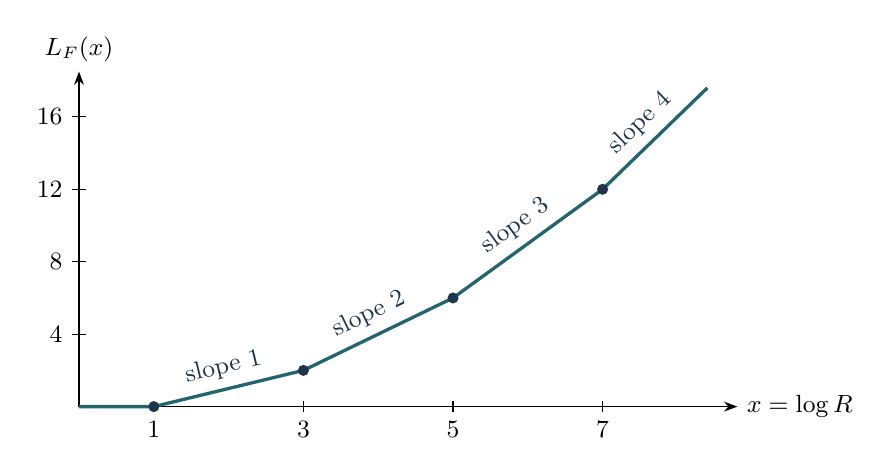
\begin{tikzpicture}[x=0.95cm,y=0.23cm,every node/.style={font=\small}]
\draw[-{Stealth}] (0,0)--(8.8,0) node[right] {$x=\log R$};
\draw[-{Stealth}] (0,0)--(0,18.5) node[above] {$L_F(x)$};
\foreach \x in {1,3,5,7} {
 \draw (\x,0.3)--(\x,-0.3) node[below] {$\x$};
}
\foreach \y in {4,8,12,16} {
 \draw (0.09,\y)--(-0.09,\y) node[left] {$\y$};
}
\draw[very thick,Accent] (0,0)--(1,0)
 --node[midway,above,sloped,text=Ink] {slope $1$} (3,2)
 --node[midway,above,sloped,text=Ink] {slope $2$} (5,6)
 --node[midway,above,sloped,text=Ink] {slope $3$} (7,12)
 --node[midway,above,sloped,text=Ink] {slope $4$} (8.4,17.6);
\foreach \x/\y in {1/0,3/2,5/6,7/12} {
 \fill[Ink] (\x,\y) circle (2pt);
}
\end{tikzpicture}
\caption{The exact radial norm profile of $F$. Each unit slope jump at an odd
positive integer records one zero on the corresponding valuation shell.
The axes are ordinary real logarithms of norms, not surreal coordinates.}
\label{fig:profile}
\end{figure}

\begin{theorem}[All zeros and their first terms]\label{thm:thetazeros}
For each integer $m\ge1$ there is exactly one zero $z_m$ of $F$ with
\begin{equation}\label{eq:zerovaluation}
 v(z_m)=-(2m-1).
\end{equation}
These are all the zeros of $F$ in $K$. They are simple and belong to the
negative part of the real-coefficient Hahn field. Writing
\[
 z_m=t^{-(2m-1)}u_m,
\]
one has $u_m\equiv-1\pmod{\mm_K}$ and, more precisely,
\begin{align}
 u_m&=-1+(-1)^m t^{m(m+1)}
              +O\!\left(t^{m(m+1)+2}\right),\label{eq:unormexp}\\
 z_m&=-t^{-(2m-1)}+(-1)^m t^{m^2-m+1}
              +O\!\left(t^{m^2-m+3}\right).\label{eq:zexp}
\end{align}
In fact $u_m\in\Z[[t^2]]\subset K$. Here $O(t^a)$ means a Hahn series of
valuation at least $a$, not an ordinary numerical estimate obtained by
substituting a small real value for $t$.
\end{theorem}
\begin{proof}
At $R=e^{2m-1}$ the minimal coefficient valuations after rescaling occur
precisely at indices $m-1,m$. Normalize by setting
\begin{equation}\label{eq:normalizedtheta}
 F_m(U)=t^{m(m-1)}F\left(t^{-(2m-1)}U\right)
       =\sum_{n\ge0}t^{(n-m)(n-m+1)}U^n.
\end{equation}
This is in $\OO_K\langle U\rangle$, and its reduction is
\[
 \red(F_m)=U^{m-1}(1+U).
\]
Thus there are exactly $m-1$ roots in the open unit disk and exactly one on its
unit shell, counted with multiplicity. The shell root has reduction $-1$ and
is simple, either by the count or by Lemma~\ref{lem:hensel}.
Rescaling gives \eqref{eq:zerovaluation}.

The disk of radius $e^{2m}$ has exactly $m$ zeros, and already contains
$z_1,\ldots,z_m$. These disks exhaust $K$, so there are no additional zeros.
Conjugation preserves $F$ and the shell and fixes its unique root; hence the
root has real Hahn coefficients. Its leading coefficient is negative, making
it a negative element in the ordered real Hahn field.

For the sharper correction work near the unit $U=-1$ and divide by the unit
power $U^{m-1}$:
\begin{equation}\label{eq:Hm}
 H_m(U)=U^{1-m}F_m(U)
       =\sum_{j\ge1-m}t^{j(j-1)}U^j.
\end{equation}
There are only finitely many negative powers. The two leading terms are
$1+U$, so $H_m'(-1)=1+O(t^2)$. At $U=-1$, pair the terms with indices
$j$ and $1-j$. Their powers of $t$ agree and their signs are opposite.
All indices from $1-m$ through $m$ cancel, leaving
\[
 H_m(-1)=\sum_{j\ge m+1}(-1)^j t^{j(j-1)}
        =(-1)^{m+1}t^{m(m+1)}
          +O\!\left(t^{m(m+1)+2}\right).
\]
The use of the Laurent function $H_m$ is local to $\vabs{U+1}<1$:
each negative power of $U=-1+V$ has a binomial expansion with integral
coefficients converging for $\vabs V<1$. The Taylor coefficients of
$F_m(-1+V)$ are in $\OO_K$, so the same holds for those of $H_m(-1+V)$.
Thus its Taylor remainder after the linear term is bounded by $\vabs V^2$.
Writing $\delta=u_m+1\in\mm_K$ and $A=m(m+1)$, the equation
$H_m(-1+\delta)=0$ has a unit linear coefficient and a quadratic remainder
of strictly smaller norm than $\delta$. Hence
$v(\delta)=v(H_m(-1))=A$, and then
\[
 \delta=-H_m(-1)/H_m'(-1)+O(t^{2A}).
\]
The reciprocal of $H_m'(-1)=1+O(t^2)$ differs from one by $O(t^2)$,
and $2A\ge A+2$. This proves \eqref{eq:unormexp}; multiplying by
$t^{-(2m-1)}$ gives \eqref{eq:zexp}. No value of $U^{-1}$ at zero,
or analyticity of $H_m$ on the entire closed unit disk, was used.

Finally use $q=t^2$ in \eqref{eq:normalizedtheta}. Every exponent
$(n-m)(n-m+1)/2$ is a nonnegative integer, and at any fixed $q$-degree only
finitely many powers of $U$ occur. Solving coefficient by coefficient for
$U=-1+\sum_{k\ge1}c_kq^k$, the coefficient of the new unknown is always the
nonzero derivative of $U^{m-1}(1+U)$ at $-1$, namely $(-1)^{m-1}$.
Induction gives $c_k\in\Z$. The resulting $q$-adic series converges in $K$
and is the same unique root. Thus $u_m\in\Z[[t^2]]$.
\end{proof}

\subsection{Low-order expansions and a simple-root residue}
The accompanying exact program obtains the following expansions, where
$q=t^2$:
\begin{align*}
 u_1={}&-1-q-2q^2-4q^3-9q^4-21q^5-52q^6+O(q^7),\\
 u_2={}&-1+q^3+3q^4+9q^5+O(q^6),\\
 u_3={}&-1-q^6-3q^7-9q^8+O(q^9),\\
 u_4={}&-1+q^{10}+3q^{11}+9q^{12}+O(q^{13}).
\end{align*}
The first row agrees with the negative of the series $\xi_0(q)$ in
Sokal's Eq.~(1.7) \cite{Sokal}; the agreement is a check of normalization, not
independent evidence for novelty. The growing first-correction exponent
$m(m+1)$ is the important scale-separation fact here.

\begin{corollary}\label{cor:thetaresidue}
At the simple zero $z_m$,
\begin{equation}\label{eq:thetaderivative}
 v\bigl(F'(z_m)\bigr)=-m^2+3m-1,
 \qquad
 \operatorname{lc}\bigl(F'(z_m)\bigr)=(-1)^{m-1}.
\end{equation}
Consequently the local residue of $\mathrm dZ/F(Z)$ at $z_m$ has valuation
$m^2-3m+1$ and leading coefficient $(-1)^{m-1}$.
\end{corollary}
\begin{proof}
Differentiating \eqref{eq:normalizedtheta} gives
\[
 F_m'(u_m)=t^{m(m-1)-(2m-1)}F'(z_m).
\]
The left side has valuation zero and reduction
$\bigl(U^{m-1}(1+U)\bigr)'_{U=-1}=(-1)^{m-1}$.
This yields \eqref{eq:thetaderivative}. The residue at a simple zero is
$1/F'(z_m)$, which reverses the valuation and inverts the leading coefficient.
\end{proof}

\subsection{The global product and coefficient identities}
Theorem~\ref{thm:canonicalproduct} now gives the complete product
\begin{equation}\label{eq:thetaprod}
 \boxed{\displaystyle
 F(Z)=\prod_{m\ge1}\left(1-\frac Z{z_m}\right).}
\end{equation}
It converges in the Gauss norm on every fixed disk. Indeed
$\vabs{z_m^{-1}}=e^{-(2m-1)}$, so each tail factor approaches one uniformly
there. There is no extra zero-free entire factor to determine, and $F(0)=1$
fixes the constant.

Comparing coefficients gives an infinite family of exact identities. For
$k\ge1$,
\begin{equation}\label{eq:symmetriczeros}
 \sum_{1\le i_1<\cdots<i_k}
   \frac1{z_{i_1}\cdots z_{i_k}}
       =(-1)^k t^{k^2}.
\end{equation}
These sums genuinely converge: below any valuation cutoff only finitely many
index tuples can occur, since $v(z_j^{-1})=2j-1$. For $k=1$ the identity is
$\sum_{m\ge1}z_m^{-1}=-t$. The smallest possible valuation on the left of
\eqref{eq:symmetriczeros} is $1+3+\cdots+(2k-1)=k^2$, as the exact right side
also shows.

If an annulus lies strictly between two successive zero shells,
\[
 e^{2m-1}<r<R<e^{2m+1},
\]
then the analytic argument principle of Section~\ref{sec:annuli} yields
\begin{equation}\label{eq:thetaargument}
 \Res_{[r,R]}\left(\frac{F'}F\dd Z\right)=m.
\end{equation}
It measures the first $m$ zeros inside the inner radius, not a number of
ordinary turns made by a path. The same integer is the slope of the radial norm
profile throughout that interval.

\subsection{Why the series is not an all-surcomplex entire function}
At the surcomplex argument $Z=t^{-\omega}$, the $n$th term of
\eqref{eq:theta} would have valuation
\[
 n^2-n\omega.
\]
These exponents strictly decrease with $n$, because consecutive differences are
$2n+1-\omega<0$. They form a set which is not well ordered. Thus the defining
family is not strongly summable at this argument. It also does not converge
in the full fine topology.

This does not rule out an unrelated or category-dependent extension of the
function. It proves the precise needed statement: the same series which is
entire over our rank-one field is not globally evaluable by its defining Hahn
sum on all of $\No[i]$. The obstruction agrees with, rather than refutes, the
repository's distinction between internal all-scale behavior and the
proper-class all-scale rigidity framework \cite{RepoFoundations}.

\section{Certified computation and the executed finite checks}
\label{sec:computation}

\subsection{The information an analytic representation must carry}
A symbolic representation of a Tate function needs more than a generator for
its coefficients. It should carry a field or coefficient domain, a coordinate
and radius, and a \emph{tail certificate}. For example, a certificate can be a
function $B(N)$ with
\[
 \inf_{n>N}\bigl(v(a_n)+n\beta\bigr)\ge B(N),
 \qquad B(N)\longrightarrow+\infty.
\]
Then truncation after degree $N$ has Gauss error at most $e^{-B(N)}$ on
$R=e^{-\beta}$. If that error is strictly below the norm of the retained
polynomial, Corollary~\ref{cor:rouche} certifies the same initial polynomial
and zero counts for the infinite function.

Such a certificate concerns the \emph{function-degree tail}. Each retained
coefficient can itself be an infinite Hahn series, whose exact comparison or
leading-term access requires a separate representation contract. This is
consistent with the capability distinctions in the repository's computer-algebra
report \cite{RepoCAS}. Neither Banach completeness nor a support theorem is a
universal finite-time algorithm for arbitrary set-theoretic input.

\subsection{An exact tail certificate for the quadratic example}
For $F_N(Z)=\sum_{n=0}^N t^{n^2}Z^n$ and $R=e^{-\beta}$, if
$N+1\ge-\beta/2$, then
\begin{equation}\label{eq:tailcertificate}
 \Gauss{F-F_N}R
 =\exp\!\left(-\bigl((N+1)^2+(N+1)\beta\bigr)\right).
\end{equation}
Indeed the quadratic $n^2+n\beta$ is increasing for integers $n\ge N+1$,
so its first omitted value is the minimum tail valuation. This is an exact
Gauss norm, not just a heuristic error estimate.

At the intermediate radius $R=e^{2m}$, the degree-$m$ truncation has its unique
minimal weighted valuation $-m^2$ at degree $m$, while the omitted tail starts
at $-m^2+1$. At the shell radius $R=e^{2m-1}$, its minimal weighted valuation
is $-m(m-1)$ and the omitted tail starts two valuation units higher. Thus degree
$m$ already certifies the disk and shell counts used in
Theorem~\ref{thm:thetazeros}. Additional terms are needed for additional root
coefficients, not to establish those counts.

\subsection{What was actually run}
The archive includes \texttt{code/verify-examples.py}, using only Python's standard
library and exact \texttt{fractions.Fraction} arithmetic. It was executed under
Python 3.13.5. The preserved report \texttt{data/verification.json} records every individual
assertion and the computed root expansions; \texttt{data/verification-summary.txt}
contains the human-readable run summary.

For each $1\le m\le8$, the program forms
\[
 G_m(U,q)=\sum_{n\ge0}q^{(n-m)(n-m+1)/2}U^n
 \pmod{q^{N_m}},\qquad N_m=\frac{m(m+1)}2+8.
\]
Only finitely many $n$ contribute at that precision. Formal Newton iteration in
$\Q[q]/(q^{N_m})$ starts at $U=-1$; its derivative has invertible constant
coefficient. The program checks the final residual exactly, the initial
constant, the vanishing of all premature correction terms, the first correction
sign, and the leading derivative coefficient.

\begin{center}\small
\begin{tabularx}{\textwidth}{@{}Lrr@{}}
\toprule
Finite check family & Assertions & Passed\\\midrule
Eight formal root expansions, five assertions each & 40 & 40\\
Displayed first-root coefficients through $q^6$ & 1 & 1\\
Active Newton indices at forty corners and forty intervals & 80 & 80\\
Quadratic-tail formula on a rational test grid & 246 & 246\\
Monomial residue-pullback exponents & 175 & 175\\\midrule
Total for this one program & 542 & 542\\\bottomrule
\end{tabularx}
\end{center}

The report is deliberately a finite-check report. It does not verify arbitrary
Hahn supports, infinite product convergence, Banach-space arguments, algebraic
closedness, the classification of Berkovich points, or de Rham cohomology in a
proof assistant. The infinite statements rely on the mathematical proofs in this
article and the explicitly cited standard inputs, not on extrapolation from
542 successful tests.

\section{Conclusions, boundaries, and natural continuations}
\label{sec:conclusion}

\subsection{What has been added to the documentation}
The main addition is a usable interface between two kinds of mathematics. The
repository's support-controlled Hahn coefficient families can be restricted to
small valuation disks; in rank one this restriction carries an explicit Banach
norm and genuine convergence. Tate algebras, in turn, sit strictly inside the
polynomial-coefficient Hahn ring, rather than being a different notation for it.
The ring chain \eqref{eq:chain} and the positive-rescaling map make both facts
precise.

Once this interface is in place, preparation turns infinite series into finite
zero geometry on every closed disk. The corresponding Berkovich points explain
why the Gauss norm, residue directions and integer Newton slopes fit together.
Analytic annuli supply a residue obstruction to primitives, but their
contractible spectra demonstrate why ordinary complex topological intuitions
must not be carried along without checking the differential-form category.
Finally the entire partial-theta example provides a single calculation in which
all these pieces interact: exact root shells, simple lifts, real ordering,
residues, a canonical product, slope counts and certified truncations.

\subsection{What is deliberately not being concluded}
No topology or analytic spectrum has been constructed on the whole proper class
$\No[i]$. No claim is made that an arbitrary set of surcomplex data is contained
in a rank-one workspace preserving its natural valuation. No coefficientwise
ordinary complex integral has been identified with a path integral in the
Berkovich spectrum. No arbitrary-radius complex exponential, global differential
field, or universal decision algorithm is supplied.

The class of entire functions here is exactly \eqref{eq:entire}; it is not a
synonym for every fine-local analytic class or for every coherent Hahn atlas in
the repository. The derivative fixes $K$. All polynomial degrees are ordinary
finite integers, all supports are sets, and all norm radii are positive ordinary
real numbers. These qualifications are mathematical hypotheses, not merely
implementation limitations.

\subsection{Three directions that now have a precise starting point}
A first continuation is several-variable Tate geometry after the explicit
rescaling map, with finite analytic maps and residues compared to the existing
multivariate Hahn-germ results. The starting ring must remain named: proving a
theorem in $K\langle Z_1,\ldots,Z_n\rangle$ does not establish it unchanged
in a radius-free Hahn-germ ring.

A second continuation is analytic curves with nontrivial skeleton graphs.
The annulus calculated here has interval skeleton and is contractible, so it is
a useful control example before studying genuine graph cycles. That extension
would use more of the standard Berkovich curve theory rather than reinterpret
an annulus as a circle.

A third continuation is a certified symbolic backend for rank-one analytic
objects, beginning with integer or rational exponent coefficient streams and
proven quadratic or linear tail bounds. It can separate root-count certificates
from root-coefficient approximations and preserve the workspace and topology as
part of an object's type. The finite program supplied here is a regression test
for that future backend, not the backend itself.

\appendix
\section{Notation and category ledger}
\label{app:notation}
\begin{longtable}{@{}P{0.29\textwidth}P{0.66\textwidth}@{}}
\toprule
Notation & Meaning\\\midrule\endhead
$\SC=\No[i]$ & The proper class of surcomplex numbers; not our Banach field.\\[0.45em]
$t^\gamma=\omega^{-\gamma}$ & Conway normal-form monomial, not an arbitrary
surreal exponential convention.\\[0.45em]
$K=\C((t^\R))$ & The fixed set-sized full Hahn field, algebraically closed and
spherically complete.\\[0.45em]
$v(a),\ \vabs a=e^{-v(a)}$ & Leading real exponent and its real-valued
multiplicative norm; every nonzero complex constant has norm one.\\[0.45em]
$R=e^{-\beta}$ & An ordinary real norm radius; scaling is performed by the
coefficient $t^\beta$, not by treating $R$ as a norm-valued coefficient.\\[0.45em]
$A_R$ & Tate algebra on the closed valuation disk of radius $R$.\\[0.45em]
$\PP,\Ag,\FF$ & Polynomial-, convergent-germ-, and formal-coefficient Hahn
families, each with a common well-ordered exponent support.\\[0.45em]
$\mathcal H(D),\ \mathcal R_1$ & Fixed ordinary disk coefficient families,
and their common-domain germ ring.\\[0.45em]
$\EE^-$ & The analytic open-unit-disk power-series ring; no common Hahn support
is required across coefficients.\\[0.45em]
$\EE(K)$ & Functions analytic on every centered closed disk of finite real norm
radius.\\[0.45em]
$\Sp(A_R),\ \zeta_{a,r}$ & A set of bounded multiplicative seminorms and a disk
seminorm, not a field element or an additional surreal number.\\[0.45em]
$A[r,R]$ & Analytic Laurent series with decay at both ends of the annulus.\\[0.45em]
$\mathrm d,\ H^1_{\dR}$ & Coordinate differentiation fixing $K$, and the
cohomology of the displayed global analytic differential complex.\\[0.45em]
$O(t^a)$ & A Hahn error of valuation at least $a$, not a numerical
specialization estimate.\\[0.45em]
$q=t^2$ & The formal grading used to compute the normalized roots $u_m$.
\\\bottomrule
\end{longtable}

\section{Reproduction and placement in the repository}
The LaTeX source is standalone: its bibliography and diagrams are embedded, and
no external image, bibliography database, font file, or repository checkout is
needed. Build it with
\begin{quote}\ttfamily\small
latexmk -pdf -interaction=nonstopmode -halt-on-error article.tex
\end{quote}
\begin{samepage}
Run the finite checks from the package directory with a separate output path:
\begin{quote}\ttfamily\small
python code/verify-examples.py --output /tmp/berkovich-verification.json
\end{quote}
\end{samepage}
The maintained article is now placed in
\begin{center}\small\texttt{docs/surcomplex/rank-one-berkovich/}\end{center}
The accompanying \texttt{repository-audit.md} records the original inspected
paths and snapshot; \texttt{build-report.md} records the delivered build.
Those historical records and the original \texttt{code/} and \texttt{data/}
files are preserved. The current \texttt{README.md} records the maintained
proof review and rebuilt PDF.

\begin{thebibliography}{99}

\bibitem{Poonen}
B. Poonen, \emph{Maximally complete fields},
L'Enseignement Math\'ematique (2) \textbf{39} (1993), 87--106.
Hahn-field construction and Corollary 4.
\href{https://math.mit.edu/~poonen/papers/amsval.pdf}{Author's full text}.

\bibitem{Temkin}
M. Temkin, \emph{Introduction to Berkovich analytic spaces},
arXiv:1010.2235, version 2 (2011).
Sections 2--3 on seminorm spectra and affinoid algebras.
\href{https://arxiv.org/abs/1010.2235v2}{pinned arXiv record};
\href{https://arxiv.org/pdf/1010.2235v2}{version 2 full text}.

\bibitem{PT}
J. Poineau and D. Turchetti, \emph{Berkovich curves and Schottky uniformization},
arXiv:2010.09043, version 1 (2020).
Part I, especially Sections I.2--I.4 and I.6--I.9.
\href{https://arxiv.org/abs/2010.09043v1}{pinned arXiv record};
\href{https://arxiv.org/pdf/2010.09043v1}{version 1 full text}.

\bibitem{Sokal}
A. D. Sokal, \emph{The leading root of the partial theta function},
Advances in Mathematics \textbf{229} (2012), 2603--2621.
\href{https://doi.org/10.1016/j.aim.2012.01.012}{doi:10.1016/j.aim.2012.01.012};
Preprint version 1 (2011), especially Eq.~(1.7):
\href{https://arxiv.org/abs/1106.1003v1}{arXiv:1106.1003v1}.

\bibitem{RepoMap}
V. Reshetnikov, \emph{Surreal repository: The surreal and surcomplex reports},
documentation catalogue, snapshot \texttt{e260237db9b7} (September 21, 2026).
\href{\repobase docs/README.md}{\texttt{docs/README.md}}.
The full commit identifier is recorded in Section~\ref{sec:gap}.

\bibitem{RepoAnalysis}
\emph{Surcomplex Analysis: Germs, coherent Hahn sections, and infinitesimal
zero geometry}, research report in the Surreal repository, same snapshot.
\href{\repobase docs/surcomplex/analysis/article.tex}{LaTeX source};
\href{\repobase docs/surcomplex/analysis/README.md}{report README}.
AI-assisted, unrefereed repository draft.

\bibitem{RepoGeometry}
\emph{Infinitesimal Analytic Geometry over the Surcomplex Numbers:
Radius-Free Germs, a Nullstellensatz, and Finite Maps}, research report,
same snapshot.
\href{\repobase docs/surcomplex/analytic-geometry/README.md}{Report README};
\href{\repobase docs/surcomplex/analytic-geometry/article.tex}{LaTeX source}.
AI-assisted, unrefereed repository draft.

\bibitem{RepoPolynomial}
\emph{Surcomplex Polynomial Algebra: Root Geometry, Newton Profiles,
Multiscale Stability, and Residue Duality}, research report, same snapshot.
\href{\repobase docs/surcomplex/polynomial-algebra/README.md}{Report README};
\href{\repobase docs/surcomplex/polynomial-algebra/article.tex}{LaTeX source}.
AI-assisted, unrefereed repository draft.

\bibitem{RepoContours}
\emph{Jordan Separation, Cauchy Theory, and Stokes Calculus on the Surcomplex
Plane}, research report, same snapshot.
\href{\repobase docs/surcomplex/contours-and-stokes/README.md}{Report README};
\href{\repobase docs/surcomplex/contours-and-stokes/article.tex}{LaTeX source}.
Includes explicit Berkovich comparisons and the intrinsic-workspace topology
qualification. AI-assisted, unrefereed repository draft.

\bibitem{RepoFoundations}
\emph{Foundations for surreal and surcomplex mathematics: Sets, classes,
universes, type theories, and a pinned Lean audit}, research report,
same snapshot.
\href{\repobase docs/foundations-and-computation/foundations/README.md}{Report README};
\href{\repobase docs/foundations-and-computation/foundations/article.tex}{LaTeX source}.
The README's two quadratic-exponent examples and its discussion of
Section 11 identify the antecedent of \eqref{eq:theta}.
AI-assisted, unrefereed repository draft.

\bibitem{RepoCAS}
\emph{Surreal and Surcomplex Numbers in Symbolic Computer Algebra}, research
report, same snapshot.
\href{\repobase docs/foundations-and-computation/computer-algebra/README.md}{Report README};
\href{\repobase docs/foundations-and-computation/computer-algebra/article.tex}{LaTeX source}.
Used for the distinction between denotation, effective coefficient access,
decision procedures and certified approximation.
AI-assisted, unrefereed repository draft.

\end{thebibliography}
\end{document}
